\documentclass[a4paper, 11pt,reqno]{article}
\input{/Users/olivierglorieux/Desktop/BCPST/2020:2021/preambule.tex}
\geometry{hmargin=1.5cm,vmargin=2.5cm }
\usepackage{enumitem}
\newif\ifshow
\showtrue
\input{/Users/olivierglorieux/Desktop/BCPST/2021:2022/ifshow.tex}



\author{Olivier Glorieux}


\begin{document}

\title{Correction - DM1 
}





\begin{exercice}(10'+40'+30'=1h20)
R\'esoudre dans $\R$ et selon les valeurs du param\`etre $m\in\R$, les in\'equations suivantes:
\begin{enumerate}
\item $x^2-(m+1)x+m\geq 0$
\item $\ddp\frac{m}{x-1} \leq \ddp\frac{1}{x+2}$
\item $\sqrt{2x+m}\geq x+1$
\end{enumerate}
\end{exercice}










\begin{correction} 
\begin{enumerate}
\item \textbf{R\'esolution dans $\mathbf{\R}$ de $\mathbf{x^2-(m+1)x+m\geq 0}$:}\\
\noindent  Ici le domaine de r\'esolution est $\R$. On calcule le discriminant et on obtient que $\Delta=(m-1)^2$. On \'etudie donc 2 cas:
 \begin{itemize}
 \item[$\bullet$] Cas 1: si $m=1$: Alors $\Delta=0$ et $x=1$ est la seule solution et $x^2-(m+1)x+m\geq 0\Leftrightarrow (x-1)^2\geq 0$. Ainsi \fbox{$\mathcal{S}_{m=1}=\R$.}
 \item[$\bullet$] Cas 2: si $m\not= 1$: alors $\Delta>0$ et les deux solutions r\'eelles distinctes sont 
 $x_1=\ddp\frac{m+1+|m-1|}{2}$ et $x_2=\ddp\frac{m+1-|m-1|}{2}$. On doit donc distinguer deux cas:
 \begin{itemize}
 \item[$\star$] Si $m<1$: les deux racines sont alors $m$ et $1$ et on obtient \fbox{$\mathcal{S}_{m<1}=\rbrack -\infty,m\rbrack\cup\lbrack 1,+\infty\lbrack$.}
 \item[$\star$] Si $m>1$: les deux racines sont alors $1$ et $m$ et on obtient \fbox{$\mathcal{S}_{m>1}=\rbrack -\infty,1\rbrack\cup\lbrack m,+\infty\lbrack$.}
 \end{itemize}
 \end{itemize}
 ---
\item \textbf{R\'esolution dans $\mathbf{\R}$ de $\mathbf{\ddp\frac{m}{x-1} \leq \ddp\frac{1}{x+2}}$:}\\
\noindent L'in\'equation est d\'efinie si $x-1\not= 0$ et $x+2\not= 0$. Ainsi, $\mathcal{D}=\R\setminus\lbrace  -2,1 \rbrace$.
Sur cet ensemble, on obtient
$$
\ddp\frac{m}{x-1}\leq \ddp\frac{1}{x+2} \Leftrightarrow  \ddp\frac{m(x+2)-(x-1)}{(x-1)(x+2)}\leq 0
\Leftrightarrow  \ddp\frac{x(m-1) +2m+1  }{(x-1)(x+2)}\leq 0.
$$
\begin{itemize}
 \item[$\bullet$] Si $m=1$, l'in\'equation \`a r\'esoudre devient alors 
$$\ddp\frac{m}{x-1}\leq \ddp\frac{1}{x+2} \Leftrightarrow  \ddp\frac{3}{(x-1)(x+2)}\leq 0.$$
Un tableau de signe donne alors : \fbox{$\mathcal{S}_{m=1}=\rbrack -2,1\lbrack$}.
\item[$\bullet$]  Si $m\not= 1$, alors la racine de $x(m-1)+2m+1$ est $\ddp\frac{2m+1}{1-m}$.
Pour pouvoir faire un tableau de signe correct, on doit savoir o\`u elle se situe par rapport \`a $-2$ et $1$.
\begin{itemize}
\item[$\star$] Si $m>1$.\\
\noindent La r\'esolution de $\ddp\frac{2m+1}{1-m}\leq -2$ est justement \'equivalente \`a $m>1$. Ainsi, la racine $\ddp\frac{2m+1}{1-m}$ est la plus petite des trois. On peut alors faire un tableau de signe, en remarquant en particulier que $m>1\Leftrightarrow m-1>0$:\\
%\begin{center}

\begin{tikzpicture}
\hspace{-1cm}
 \tkzTabInit[lgt=4]{ $x$          /1,%
      % $\sin{x}$     /1,%
    $(m-1)x+2m+1$     /1,
       $x+2$    /1,
       $x-1$            /1,
        $\ddp\frac{(m-1)x+2m+1}{(x-1)(x+2)}$              /1}%
     { $-\infty$ , $\frac{2m+1}{1-m}$ ,$-2$ , $1$ ,$+\infty$}%
  \tkzTabLine {,$-$,0,$+$,t,$+$,t,$+$,}%
  \tkzTabLine{ ,$-$,t,$-$,0,$+$,t,$+$,}
   \tkzTabLine{ ,$-$,t,$-$,t,$-$,0,$+$,}
\tkzTabLine{,$-$,0, $+$,d, $-$,d, $+$,}
\vspace{0.5cm}
\end{tikzpicture}
\vspace{0.5cm}\\
%\end{center}
Ainsi, \fbox{$\mathcal{S}_{m>1}=\left\rbrack -\infty,\ddp\frac{2m+1}{1-m}\right\rbrack\cup \; \rbrack -2,1\lbrack$}.
\item[$\star$] Si $0\leq m <1$.\\
La r\'esolution de $\ddp\frac{2m+1}{1-m}\geq 1$ est \'equivalente \`a $0\leq m<1$.
Ainsi,  la racine $\ddp\frac{2m+1}{1-m}$ est la plus grande des trois. On peut alors faire un tableau de signe, en remarquant en particulier que $m<1\Leftrightarrow m-1<0$:
\begin{center}
\begin{tikzpicture}
\hspace{-1cm}
 \tkzTabInit[lgt=4]{ $x$          /1,%
     %  $\sin{x}$     /1,%
     $(m-1)x+2m+1$      /1,
       $x+2$    /1,
       $x-1$            /1,
        $\ddp\frac{(m-1)x+2m+1}{(x-1)(x+2)}$               /1}%
     { $-\infty$ ,$-2$ , $1$ ,$\ddp\frac{2m+1}{1-m}$,$+\infty$}%
  \tkzTabLine {,$+$,t,$+$,t,$+$,0,$-$,}%
  \tkzTabLine{ ,$-$,0,$+$,t,$+$,t,$+$,}
   \tkzTabLine{, $-$,t,$-$,0,$+$,t,$+$,}
\tkzTabLine{,$+$,d, $-$, d, $+$, 0, $-$,}
\vspace{0.5cm}
\end{tikzpicture}
\end{center}
\vspace{0.5cm}
Ainsi, \fbox{$\mathcal{S}_{m \in [0,1[}=\rbrack -2,1\lbrack \; \cup\left\lbrack \ddp\frac{2m+1}{1-m},+\infty\right\lbrack$}.

\item[$\star$] Si $m<0$.\\
\noindent Ainsi, la racine $\ddp\frac{2m+1}{1-m}$ est entre les racines $-2$ et $1$. On peut alors faire un tableau de signe, en remarquant en particulier que $m<0<1\Rightarrow m-1<0$:
\begin{center}
\begin{tikzpicture}
\hspace{-1cm}
 \tkzTabInit[lgt=4]{ $x$          /1,%
       %$\sin{x}$     /1,%
      $(m-1)x+2m+1$       /1,
       $x+2$    /1,
       $x-1$            /1,
        $\ddp\frac{(m-1)x+2m+1}{(x-1)(x+2)}$               /1}%
     { $-\infty$ ,$-2$ ,$\ddp\frac{2m+1}{1-m}$, $1$  ,$+\infty$}%
  \tkzTabLine {,$+$,t,$+$,0,$-$,t,$-$,}%
  \tkzTabLine{ ,$-$,0,$+$,t,$+$,t,$+$,}
   \tkzTabLine{ ,$-$,t,$-$,t,$-$,0,$+$,}
\tkzTabLine{,$+$,d, $-$, 0, $+$,d, $-$,}
\vspace{0.5cm}
\end{tikzpicture}
\end{center}
\vspace{0.5cm}
Ainsi, \fbox{$\mathcal{S}_{m<0}=\left\rbrack \ddp -2,\frac{2m+1}{1-m}\right\rbrack\cup \; \rbrack 1,+\infty\lbrack$}.
\end{itemize}
\end{itemize}
---
\item \textbf{R\'esolution dans $\mathbf{\R}$ de $\mathbf{\sqrt{2x+m}\geq x+1}$:}\\
\noindent \begin{itemize}
 \item[$\bullet$] Domaine de r\'esolution:\\
L'in\'equation a un sens si: $2x+m\geq 0\Leftrightarrow x\geq -\ddp\frac{m}{2}$. Ainsi, $\mathcal{D}=\left\lbrack -\ddp\frac{m}{2},+\infty\right\lbrack$.
\item[$\bullet$] R\'esolution:\\
\begin{itemize}
\item[$\star$] Cas 1: $x+1< 0\Leftrightarrow x< -1$:\\
\noindent L'in\'equation est alors toujours v\'erifi\'ee car une racine carr\'ee est toujours positive.\\
\noindent Pour trouver l'ensemble solution, il faut alors \'etudier la position de $-\ddp\frac{m}{2}$ par rapport \`a $-1$.
$$
-\ddp\frac{m}{2}\leq -1  \Leftrightarrow  -m\leq -2\Leftrightarrow  m\geq 2.$$
Ainsi, on obtient
\begin{itemize}
\item[$\circ$] Si $m\geq 2$, alors $\mathcal{S}_{1, m\geq 2}=\left\lbrack -\ddp\frac{m}{2},-1\right\lbrack$.
\item[$\circ$] Si $m<2$, alors $\mathcal{S}_{1,m<2}=\emptyset$.
\end{itemize}
\item[$\star$] Cas 2: $x+1\geq 0\Leftrightarrow x\geq -1$:\\
\noindent Les deux termes de l'in\'equation sont alors positifs, on peut donc passer au carr\'e tout en conservant l'\'equivalence et on obtient
$$
\sqrt{2x+m}\geq x+1 \Leftrightarrow  2x+m\geq x^2+2x+1\Leftrightarrow x^2+1-m\leq 0.$$
Le discriminant est $\Delta=4(m-1)$, on a donc
\begin{itemize}
\item[$\circ$] Si $m<1$, alors $\Delta<0$ et $\mathcal{S}_{2,m<1}=\emptyset$.
\item[$\circ$] Si $m\geq 1$, alors les deux solutions sont $-\sqrt{m-1}$ et $\sqrt{m-1}$.
Il faut alors \'etudier la position de $-\sqrt{m-1}$ par rapport \`a $-\ddp\frac{m}{2}$ et \`a $-1$.
On a
$$\begin{array}{llll}
-\sqrt{m-1}\geq -\ddp\frac{m}{2}&\Leftrightarrow &\sqrt{m-1}\geq \ddp\frac{m}{2} &  \vsec\\
&\Leftrightarrow  & m^2-4m+4\geq 0 & \hbox{car les deux termes sont positifs}\vsec\\ 
&\Leftrightarrow & (m-2)^2\geq 0 & \hbox{toujours vrai.}
\end{array}$$
Ainsi, on a, pour $m\geq 1$, $-\sqrt{m-1}\geq -\ddp\frac{m}{2}$.\\
\noindent Un raisonnement analogue montre que
$$-\sqrt{m-1}\leq -1\Leftrightarrow m\geq 2.$$
\end{itemize}
On en d\'eduit les r\?esultats suivants :
\begin{itemize}
\item[$\circ$]  Si $1\leq m<2$, alors $-\sqrt{m-1}>-1$, $-\ddp\frac{m}{2}>-1$ et $-\sqrt{m-1}\geq -\ddp\frac{m}{2}$, donc $\mathcal{S}_{2,m\in [1,2[}=\lbrack -\sqrt{m-1},\sqrt{m-1}\rbrack$.
\item[$\circ$]  Si $m\geq 2$, alors  $-\sqrt{m-1}\leq -1$, $-\ddp\frac{m}{2}\leq -1$ et $-\sqrt{m-1}\geq -\ddp\frac{m}{2}$, donc $\mathcal{S}_{2,m\geq2}=\lbrack -1,\sqrt{m-1}\rbrack$.
\end{itemize}
\item[$\star$]  
On peut alors conclure:
\begin{itemize}
\item[$\circ$]  Si $m<1$, alors \fbox{$\mathcal{S}_{m<1}=\emptyset$.}
\item[$\circ$]  Si $1\leq m<2$, alors $\mathcal{S}_{m\in [1,2[} = \emptyset \cup \lbrack -\sqrt{m-1},\sqrt{m-1}\rbrack,$ soit \fbox{$\mathcal{S}_{m\in [1,2[}=\lbrack -\sqrt{m-1},\sqrt{m-1}\rbrack$}.
\item[$\circ$]  Si $m\geq 2$, alors $\mathcal{S}_{m\geq2}= \lbrack -\ddp\frac{m}{2},-1\lbrack \, \cup \, \lbrack -1,\sqrt{m-1}\rbrack,$ soit \fbox{$\mathcal{S}_{m\geq2}=\left\lbrack -\ddp\frac{m}{2},\sqrt{m-1}\right\rbrack$}.
\end{itemize}
\end{itemize}
\end{itemize}
---

\end{enumerate}
\end{correction}





%%%%%%

\begin{exercice}(5'+10'+1'+5'+30'+10'=1h01)
On considère l'équation suivante d'inconnue $x\in \R : $ 
$$\floor{2x-\sqrt{5x-1}} =0 \quad \quad (E)$$
\begin{enumerate}
\item Déterminer le domaine de définition de $(E)$. 
\item Dire si les réels suivants sont solutions ou non de $(E)$
$$x_1 = \frac{1}{5}, \, x_2 = \frac{1}{2}, \, x_3 =1,\, x_4=12$$
\item Pour tout $a\in \R$, rappeler  un encadrement de la partie entière de $a$ en fonction de $a$. 
\item Montrer que résoudre $(E)$ est équivalent à résoudre le système :
$$\left\{\begin{array}{clc}
\sqrt{5x-1} >&2x-1 &\quad(E_1)\\ 
\sqrt{5x-1} \leq &2x&\quad(E_2)
\end{array}\right.
$$
\item Résoudre les deux inéquations obtenues à la question précédente. 
\item Résoudre $(E)$. 
\end{enumerate}
\end{exercice}
\begin{correction}
\begin{enumerate}
\item Seule la fonction $x\mapsto \sqrt{x}$ n'est pas définie sur $\R$ mais sur $\R_+$ ainsi $(E)$ est bien définie pour tout $x$ tel que $5x-1\geq 0$ c'est-à-dire 
\conclusion{ $D_E=]\frac{1}{5},+\infty[$}
\item Cours 
\conclusion{$\forall a\in \R\, \quad  a-1 <\floor{a}\leq a$}

\item Notons $f(x) = \floor{2x-\sqrt{5x-1} }$ 
On a $f(\frac{1}{5}) = \floor{2\frac{1}{5}-\sqrt{5\frac{1}{5}-1} }= \floor{2\frac{1}{5}} =0$
Donc \conclusion{$\frac{1}{5}$ est solution de $E$}

On a $f(\frac{1}{2} )  =\floor{2\frac{1}{2}-\sqrt{5\frac{1}{2}-1} } = \floor{1-\sqrt{\frac{3}{2} }}$ Or $\frac{3}{2}> 1 $ donc 
$\sqrt{\frac{3}{2}} >\sqrt{1}=1$ et donc 
$1-\sqrt{\frac{3}{2} }<0$ ainsi  
\conclusion{$\frac{1}{2}$ n'est pas solution de $E$}

On a $f(1) = \floor{2\times 1-\sqrt{5-1}} =\floor{2-2}=\floor{0}$
\conclusion{$1$ est solution de $E$}

On  a $f(12) = \floor{2\times 12-\sqrt{60-1}}=\floor{24-\sqrt{59}}$ 
Or$ 59<64=8^2$ donc  $\sqrt{59} < 8 $ et 
$24-\sqrt{59}> 24-8=16$ ainsi $f(2)>16 $ et 
\conclusion{$12$ n'est pas solution de $E$}


\item D'après ce qu'on vient de voir, pour tout $x\in D_E$ on a :
$$2x-\sqrt{5x-1} -1<\floor{2x-\sqrt{5x-1} } \leq 2x-\sqrt{5x-1} $$
Si $x$ est solution de $(E)$ on a $\floor{2x-\sqrt{5x-1} }=0$ et donc l'équation $(E)$ équivaut à $2x-\sqrt{5x-1} -1<0 \leq 2x-\sqrt{5x-1} $, soit 
\conclusion{$\left\{\begin{array}{clc}
\sqrt{5x-1} >&2x-1 &\quad(E_1)\\ 
\sqrt{5x-1} \leq &2x&\quad(E_2)
\end{array}\right.
$}

\item Résolvons ces deux inéquations. Tout d'abord la première :
$$\sqrt{5x-1} >2x-1 \quad(E_1)$$
On distingue deux cas : 
\begin{itemize}
\item[$\blacktriangleright$] \underline{Cas 1 :} $2x-1\geq 0$ c'est-à-dire $x\geq \frac{1}{2}$

Alors on peut passer au carré dans l'équation car les deux cotés sont du même signe. On a alors : 
\begin{align*}
(E_1)& \equivaut 5x-1 > (2x-1) ^2\\
& \equivaut 5x-1 > 4x^2-4x+1\\
& \equivaut 4x^2-9x+2<0
\end{align*}
Un petit discriminant comme on aime : 
$\Delta = 9^2 - 4*4*2 = 81- 32= 49 =7^2$. 
$4x^2-9x+2$ admet donc deux racines 
$$r_1 = \frac{9+7}{8}=2 \quadet r_2 =\frac{9-7}{8} = \frac{1}{4}$$

Ainsi les solutions de $(E_1) $ sur $[\frac{1}{2},+\infty[$ sont
\begin{align*}
\cS_1 &= ]\frac{1}{4},2[ \cap [\frac{1}{2},+\infty[ \cap D_E\\
		 &= [\frac{1}{2},2[	
\end{align*}


\conclusion{  Les solutions de $(E_1) $ sur $[\frac{1}{2},+\infty[$ sont  $\cS_1 = [\frac{1}{2},2[	$}

\item[$\blacktriangleright$] \underline{Cas 2 :} $2x-1<0$ c'est-à-dire $x<\frac{1}{2}$

Dans ce cas, tous les réels $x\in D_E$ sont solutions car le membre de gauche est positif et celui de droite négatif. 

\conclusion{  Les solutions de $(E_1) $ sur $]-\infty,\frac{1}{2}[$ sont  $\cS_1' = [\frac{1}{5},\frac{1}{2}]	$}

En conclusion :
\conclusion{  Les solutions de $(E_1) $ sur $D_E$ sont  $\cS = \cS_1\cup \cS_1' = [\frac{1}{5},2[	$}



\end{itemize}

On fait la même chose pour $(E_2) $ 
$$\sqrt{5x-1} \leq 2x \quad(E_2)$$

On distingue deux cas : 
\begin{itemize}
\item[$\blacktriangleright$] \underline{Cas 1 :} $2x\geq 0$ c'est-à-dire $x\geq 0$

Alors on peut passer au carré dans l'équation car les deux cotés sont du même signe. On a alors : 
\begin{align*}
(E_1)& \equivaut 5x-1 \leq  (2x) ^2\\
& \equivaut 5x-1 \leq 4x^2\\
& \equivaut 4x^2-5x+1\geq 0
\end{align*}
Un petit discriminant comme on aime : 
$\Delta = 5^2 - 4*4*1 = 25- 16= 9 =3^2$. 
$4x^2-5x+1$ admet donc deux racines 
$$r_1 = \frac{5+3}{8}=1 \quadet r_2 =\frac{5-3}{8} = \frac{1}{4}$$

Ainsi les solutions de $(E_2) $ sur $[0,+\infty[$ sont
\begin{align*}
\cE_2 &=( ]-\infty, \frac{1}{4}] \cup [1,+\infty[) \cap [0,+\infty[ \cap D_E\\
		 &= [\frac{1}{5} ,\frac{1}{4}] \cup[1,+\infty[	
\end{align*}


\conclusion{  Les solutions de $(E_2) $ sur $[0,+\infty[$ sont  $\cE_2 =  [\frac{1}{5} ,\frac{1}{4}] \cup[1,+\infty[	$}

\item[$\blacktriangleright$] \underline{Cas 2 :} $2x<0$ c'est-à-dire $x<0$

Dans ce cas, aucun réel n'est solution car le membre de gauche est positif et celui de droite négatif. 

\conclusion{  Les solutions de $(E_2) $ sur $]-\infty,0[$ sont  $\cE_2' =\emptyset$}

En conclusion :
\conclusion{  Les solutions de $(E_2) $ sur $D_E$ sont  $\cE = \cE_2\cup \cE_2' =  [\frac{1}{5} ,\frac{1}{4}] \cup[1,+\infty[		$}



\end{itemize}

\item $x$ est solution de $(E)$ si et seulement si il est solution de $(E_1) $ et $(E_2)$, l'ensemble des solutions correspond donc à l'intersection : $\cE \cap \cS =   ([\frac{1}{5} ,\frac{1}{4}] \cup[1,+\infty[	) \cap[\frac{1}{5},2[ = 
[\frac{1}{5} ,\frac{1}{4}] \cup[1,2[$ 

\conclusion{ Les solutions de $(E)$ sont $[\frac{1}{5} ,\frac{1}{4}] \cup[1,2[$ }


\end{enumerate}
\end{correction}



\end{document}
